\documentclass[10pt,a4paper]{jarticle}
\usepackage{docmute}
\usepackage{tc2016_utf}
\usepackage[dvipdfmx]{graphicx,color}
\usepackage[fleqn]{amsmath}
\usepackage{algorithm,algorithmic}
\usepackage{amssymb,epsfig}
\usepackage{ascmac}

\usepackage{url}
\usepackage{bm}
\usepackage{ascmac}
\usepackage{pifont}
%\usepackage{multirow}
\usepackage{enumerate}
%\usepackage{cases}
\usepackage{type1cm}
\usepackage{here}
\usepackage{secdot}
\sectiondot{subsection}
\sectiondot{subsubsection}

\input{jdummy.def}

\def\vec#1{\mbox{\boldmath$#1$}}
\def\vector#1{\mbox{\boldmath $#1$}}

\newcommand{\argmax}{\mathop{\rm arg~max}\limits}
\newcommand{\argmin}{\mathop{\rm arg~min}\limits}
\newcommand{\umax}{\mathop{\rm max}\limits}

\def\R{{\Bbb R}}
\def\Z{{\Bbb Z}}

\renewcommand{\topfraction}{0.8}
\renewcommand{\bottomfraction}{0.8}
\renewcommand{\dbltopfraction}{0.8}
\renewcommand{\textfraction}{0.1}
\renewcommand{\floatpagefraction}{0.8}
\renewcommand{\dblfloatpagefraction}{0.8}
\setcounter{topnumber}{3}
\setcounter{bottomnumber}{3}
\setcounter{totalnumber}{3}
\begin{document}
\section{KIT-C3の構成}
\subsection{ハードウェア構成}
\subsubsection{ハードウェア}
本ロボットでは,シニアカータウンカート(スズキ株式会社製TC1A4)の走行系を用いた.シニアカーの走行系は,バッテリーや走行安定性,防水性など,様々な面で屋外での走行機能の信頼性が高く,故障などの問題の発生率が低い.さらに,ホイールレングスが1[m]程度あるため,直進走行性能が高く,自動走行制御に対して再現性が高いというアドバンテージがある.一方で,つくばチャレンジの他チームの小型走行ロボットよりは比較的車体が大きく,車重も97[kg]と重い.また,シニアカーの座席下部分には自律走行をさせるにあたって必要なマイコンや電源装置が収められている.Fig.にKIT-C3の全体図を示す.

また,ステアリングの操作のためにオリエンタルモータ社製のステッピングモータをステアリング軸にギアを介して取り付けている.
自律走行時には3Dプリンタで作成したカバーを取り付けている.

\begin{figure}[bt]
 \centering
 \includegraphics[width=6cm]{./fig/png/thirdrobot_2016ver.png}
 \caption{KIT-C3の全体図}
\end{figure}


\subsubsection{センサ}
KIT-C3 は環境観測用センサとして前方下部に LRF (北陽電機製UTM-30LX)を1台,後方に同様のLRFを1台搭載している.探索対象の発見のために前方上部に3DLIDAR(北陽電機製YVT-X002)を1台取り付けた.また,ロボットの状態観測用センサとしてロータリーエンコーダ(MUTOH製UM-125)をステアリング軸に1つ取り付けている.このセニアカーの後輪は独立に2つのモータとエンコーダが搭載されており,そのエンコーダ情報をiXis Research社製マイコンボード iMCs01 により取得している.

\subsubsection{ロボットへの指令}
ロボットへの速度指令はロータリーエンコーダの処理用マイコンとして搭載した iXs Research 社のiMCs01を利用した.iMCs01で0-5[V]の電圧を生成しシニアカーのアクセル信号部に印加することで速度指令を実現している.またステアリング操舵のためのステッピングモータはArduino Unoを介して制御している.iMCs01とArduino Unoは制御用PCにUSBで接続し,制御用PCのOSはUbuntu 14.04を使用した.

\subsection{ソフトウェア構成}
\subsubsection{ROS}
ロボットの開発にはROS\cite{ros}を導入している.これはソフトウェアの再利用性を意識したものである.実際,KIT-C3で開発したソフトウェアを同チームが開発したKIT-C4やKIT-C5などの他のロボットでソフトウエア再利用することが可能であり,開発時間の短縮を図ることができる.また,ROSを用いることでデバッグや可視化に有効なツールだけでなく,世界中の開発者が作成したライブラリを容易に利用することができる.

\subsubsection{走行手法}
自律走行には,ROSのnavigationスタックを利用した.予め環境地図を作成し,環境地図上にWaypointを1メートル毎に設定し,それらを順に辿っていくようにして自律移動を行った.Waypointの設定はROSの可視化ソフトウェアrviz上でクリックやドラッグ操作で設定できるパッケージを開発しこれを用いた.経路生成および障害物回避にはmove\_baseパッケージを用いた.また,自己位置推定にはAMCL(AdaptiveMontecalro Localization)を用いた.今年も昨年と同様に前方と後方に取り付けた2台のLRFで自己位置推定を行った.また,グローバルパスプランニングにはcarrot\_planerを用いた.これはデフォルトのNavfnのグローバルプランナーでは人物発見の際に問題が生じたためである.また,ローカルプランナーにはDWAローカルプランナーを利用した.いずれも,ROSではmove\_baseのプラグインとして提供されているため簡単に利用することが出来る.
本番では人物探索を行うことが出来なかったが,人物探索についても準備を行った.予め設定したwaypointに探索エリアに関する情報を保持しておき,waypointの切替時に探索エリアかつ探索対象を発見して場合に探索対象候補へのアプローチを行った.探索対象の検出方法については\ref{200657_7Dec16}章で説明する.

\subsubsection{環境地図}
環境地図はROSのパッケージ化されたgmappingを用いて作成した.昨年は前後2台のLRFのデータを利用して地図作成を行ったが,今年は前方に取り付けたLRFのみで地図作成を行った.これはロボット後方のLRFの位置がつくば到着後に傾いたままデータを取ってしまったためである.環境地図は5[cm]四方の占有格子地図とした.また,確認走行を完了したあとは大清水公園と同公園の外でそれぞれ地図を作成し画像編集ソフトを用いて1つに統合したものを用いた.作成した地図は\ref{sec:remote_monitor}章のFig.\ref{monitor}に示す.遠隔監視システムの説明のために緑のマークが重ねてある.

\subsection{全体の構成}
これまでに説明した構成をFig.\ref{184559_7Dec16}にまとめた.ここで,ソフトウエアの枠の中には利用したROSのパッケージ群を掲載している.座標変換を行うtfなどは省略している.
\begin{figure*}[ht]
 \centering
 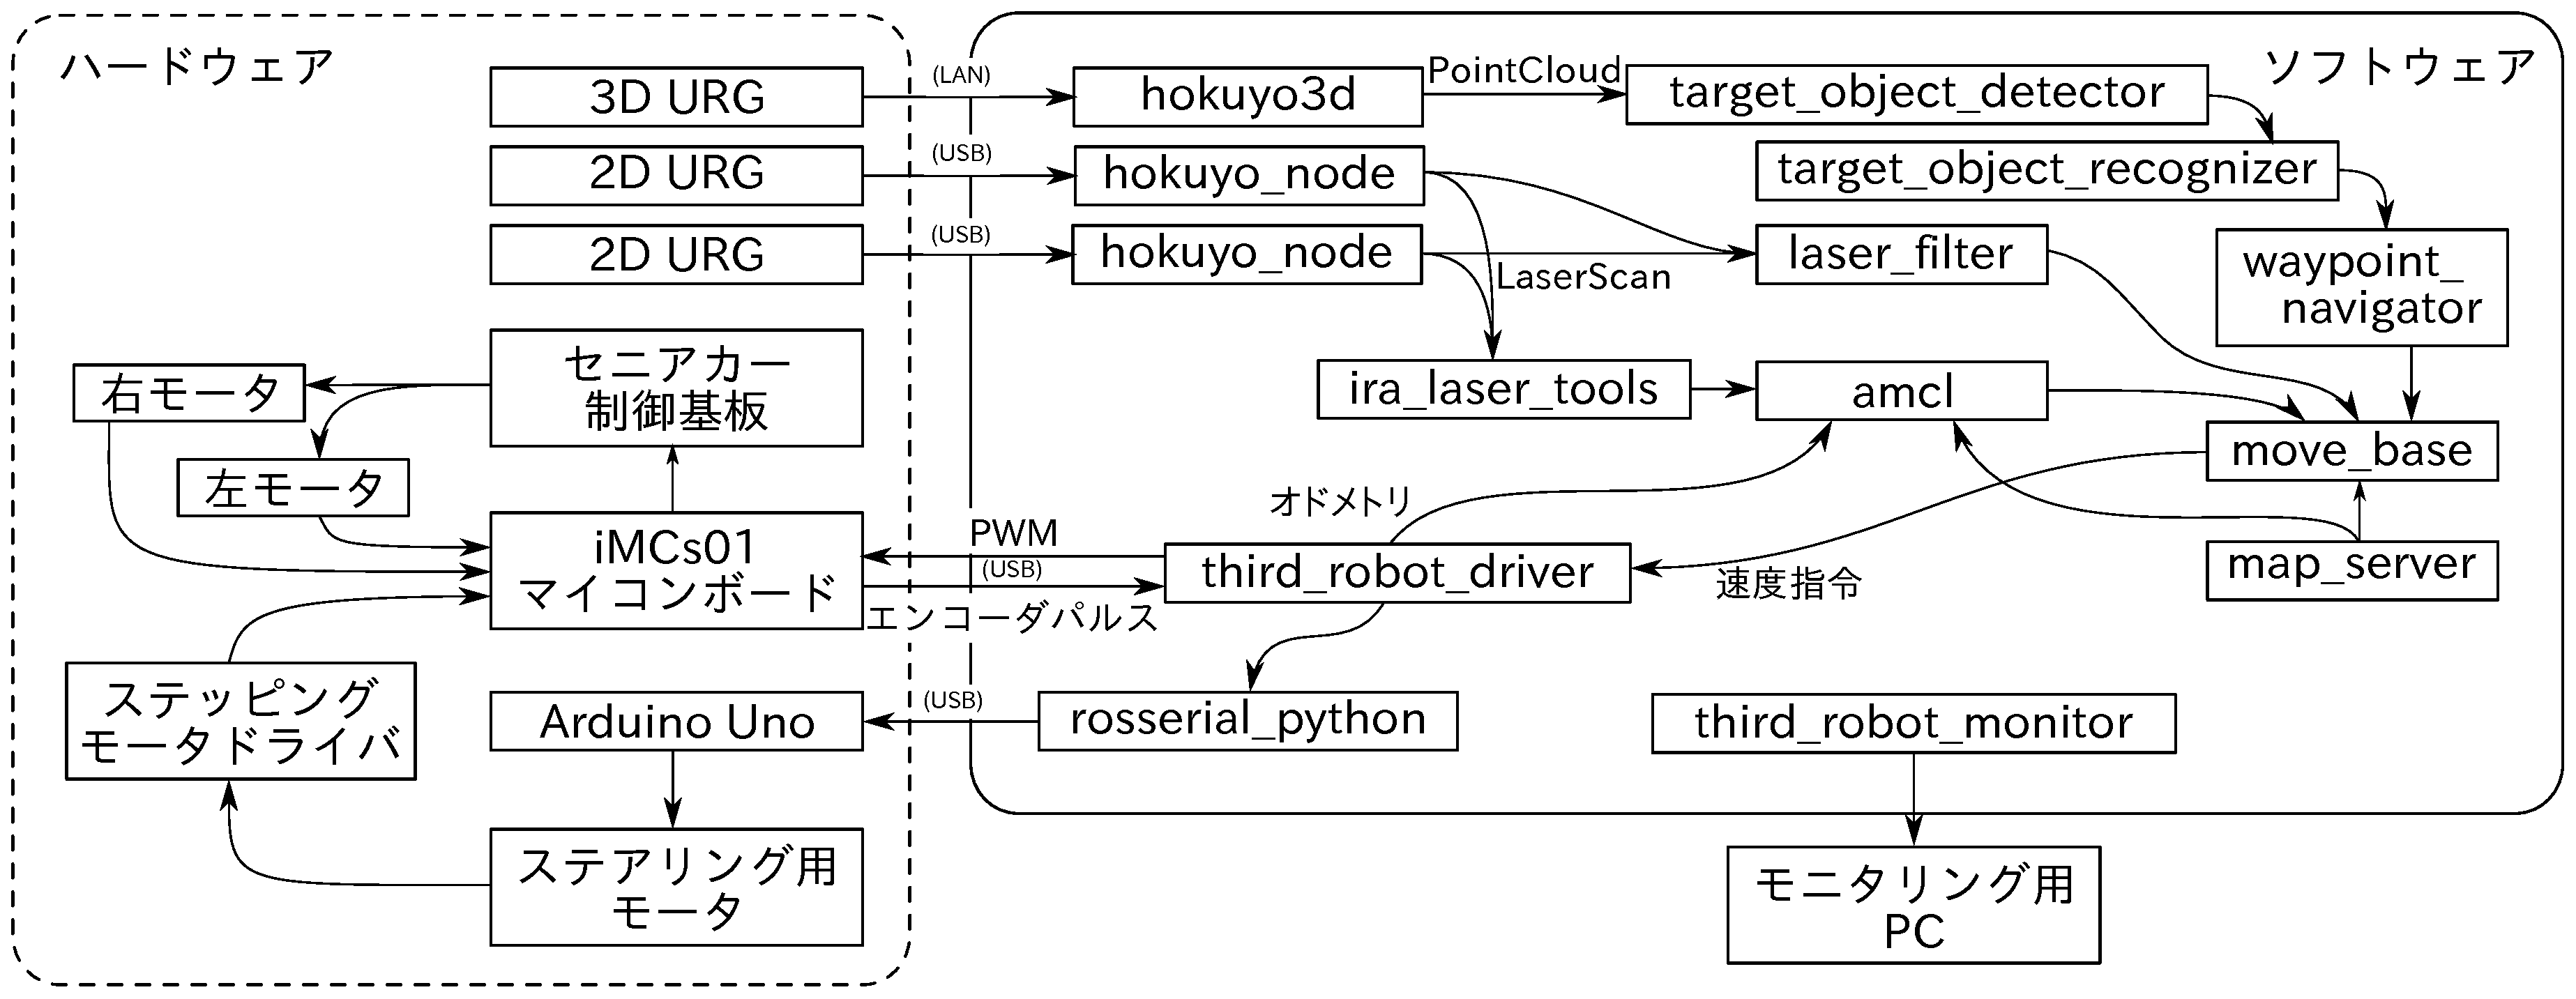
\includegraphics[width=16cm]{./fig/eps/whole_system.eps}
 \caption{KIT-C3の全体のシステム構成}
 \label{184559_7Dec16}
\end{figure*}

\end{document}

% Local Variables:
% mode: yatex
% TeX-master: "tc2016_third"
% End: